\documentclass[12pt]{article}
\usepackage{graphicx}
%\usepackage{subfigure}
\usepackage{color}

\addtolength{\textwidth}{3cm}
\addtolength{\hoffset}{-1.5cm}
\addtolength{\textheight}{3.0cm}
\addtolength{\voffset}{-1.5cm}


%\usepackage{geometry} % see geometry.pdf on how to lay out the page. There's lots.
%\geometry{letterpaper} % or letter or a5paper or ... etc
% \geometry{landscape} % rotated page geometry

% See the ``Article customise'' template for come common customisations

\title{HPS DAQ Operations Manual v2.3.4}
\author{Per Hansson Adrian, Omar Moreno, Sergey Boiarinov\thanks{Contact person for document.}, Nathan Baltzell, Sho Uemura }
%\date{} % delete this line to display the current date

%%% BEGIN DOCUMENT
\begin{document}

\maketitle

\tableofcontents

\section{System Description}
The HPS experiment data acquisition (DAQ) handles the acquisition of data for the two sub-detectors: the SVT,  and the ECal. HPS employs two DAQ architectures: the SVT is readout with Advanced Telecom Communications Architecture (ATCA) hardware while the ECal use VXS based hardware. The trigger system receives input from the ECal, and distributes a trigger signal to all detector subsystems to read out a selected event. Figure~\ref{fig:daq} gives a schematic block diagram of the DAQ system.

For the ECal, every VXS crate contains a Readout Controller (ROC) that collects digitized information, processes it, and sends it on to the Event Builder (EB). The ROC is a single blade Intel-based CPU module running DAQ software under CentOS Linux OS. For the SVT ATCA system, a multi-ROC setup runs on embedded processors situated on the ATCA main board. The EB assembles information from the SVT and ECal ROCs into a single event which is passed to the Event Recorder (ER) that writes it to a RAID5-based data storage system. The DAQ network system is a Foundry router providing high-speed connections between the DAQ components and to the JLab computing facility. 

\newpage
\section{DAQ Control}
\label{sec:daq_control}

\subsection{Starting the DAQ from scratch}\label{sec:daqstart}

\begin{enumerate}
\item 
Log into \texttt{clondaq3} as \texttt{clasrun}.
\item 
To start all DAQ processes, open a terminal and run:\newline
\texttt{> runcontrol -rocs}\newline
\end{enumerate}

This opens up all windows needed on the current workspace. The workspace should look like Fig.~\ref{fig:coda}.

It is important to be able to see all the roc terminals.  To do so it may be necessary to click on the {\bf rocs} button in the top right corner to make the roc terminals visible.

{\em Note:  if the roc terminals are oddly sized or not displaying properly, try slightly resizing the window.}
%=======================
\begin{figure}[htbp]
\begin{center}
    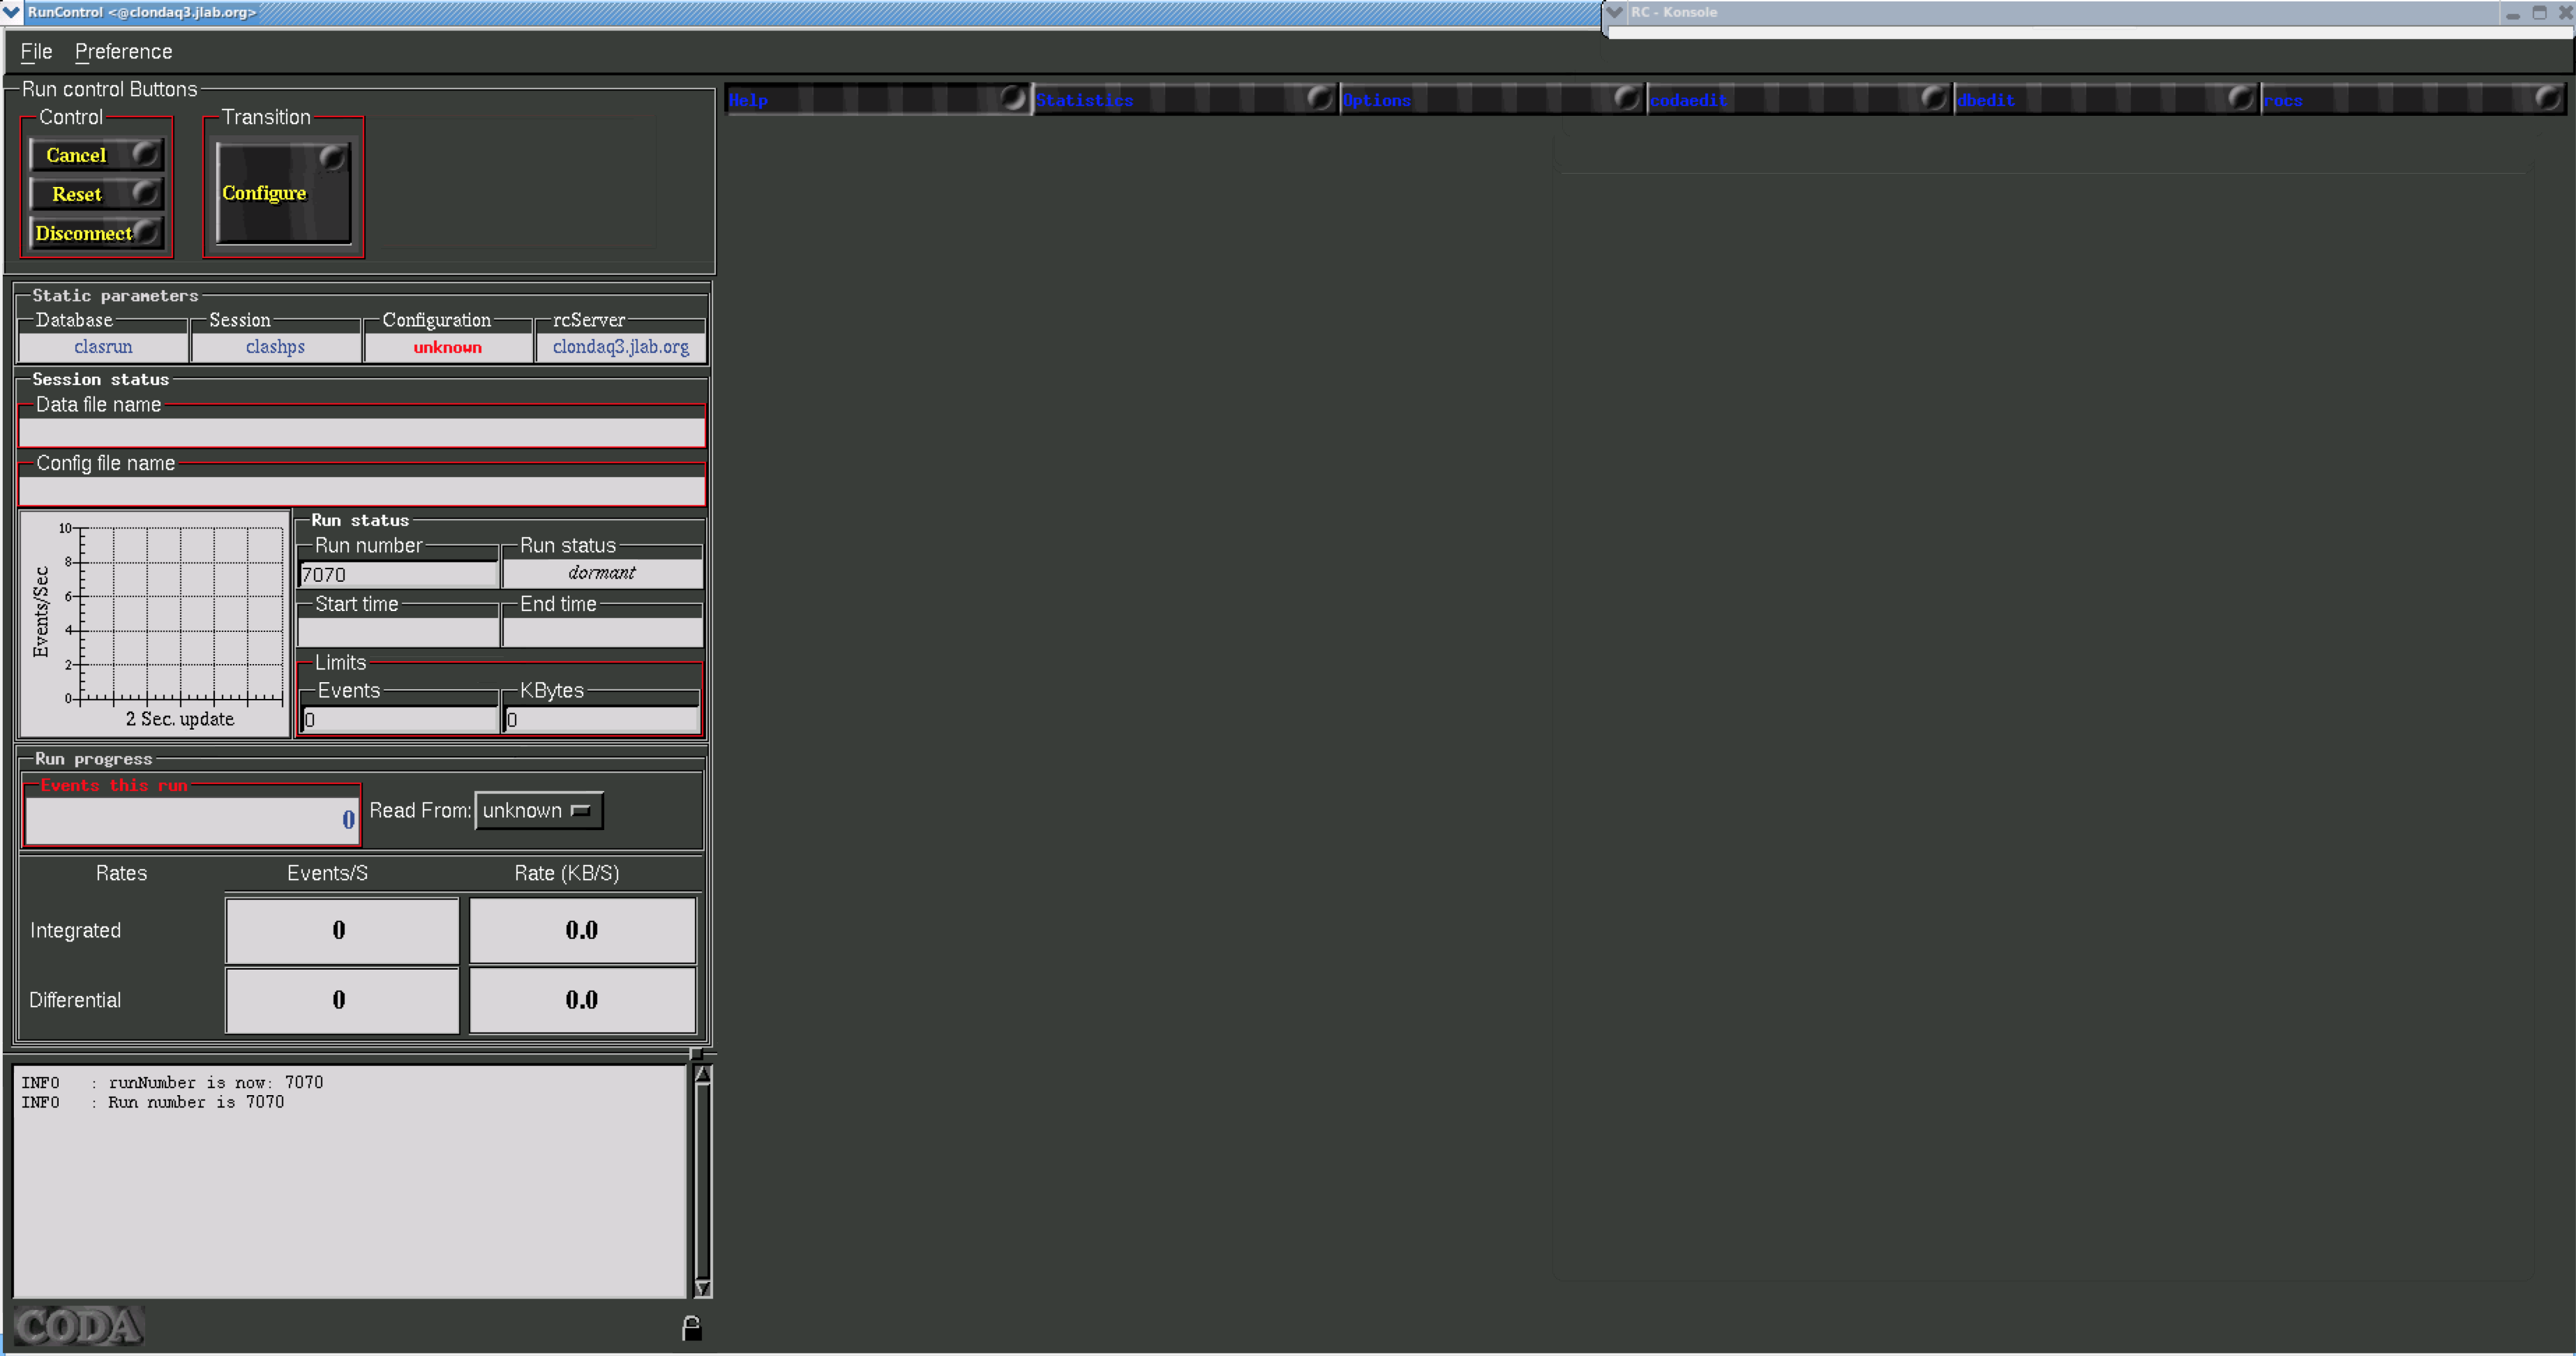
\includegraphics[width=\textwidth]{runcontrol_start.png}
\caption{CODA workspace.}
\label{fig:coda}
\end{center}
\vspace*{-5mm}
\end{figure}
%=======================

\subsection{Killing the DAQ}\label{sec:daqexit}
First, in the runcontrol GUI, click ``File''$\to``$Exit''.  You may have to do that twice.

Then, to ensure that all underlying processes are gone, log into \texttt{clondaq3} as \texttt{clasrun}, {\em being sure you are on the correct host}, and then execute the two commands:\newline
\texttt{> killall rcServer}\newline
\texttt{> killall rocs}\newline
%\texttt{> hps\_exit}\newline
%\texttt{> roc\_xterms\_exit}\newline
%This does not have to be done from the same terminal used for Section \ref{sec:daqstart}.  Do not proceed with DAQ operations until all the windows in Fig.~\ref{fig:coda} have disappeared.

\subsection{Start and stop a run}
\label{sec:startstop}

\begin{enumerate}
\item
Beamline checklist
\begin{enumerate}
\item
Beam conditions are ready for running (see beam line manual for more details).
\end{enumerate}
\item    ECal Checklist
\begin{enumerate}
\item
All HV are on.
\item
ECal monitoring app is running.
\item
ECal FADC scaler display is running.
\end{enumerate}
\item
\label{item:svt-checklist}
SVT Checklist \newline

{\bf \textcolor{red}{
For most of the steps below use the SVT summary GUI from Fig.~\ref{fig:svt_summary_gui} which can be started from the SVT sub-menu in the 
main EPICS control GUI.}}
%=======================
\begin{figure}[htbp]
\begin{center}
    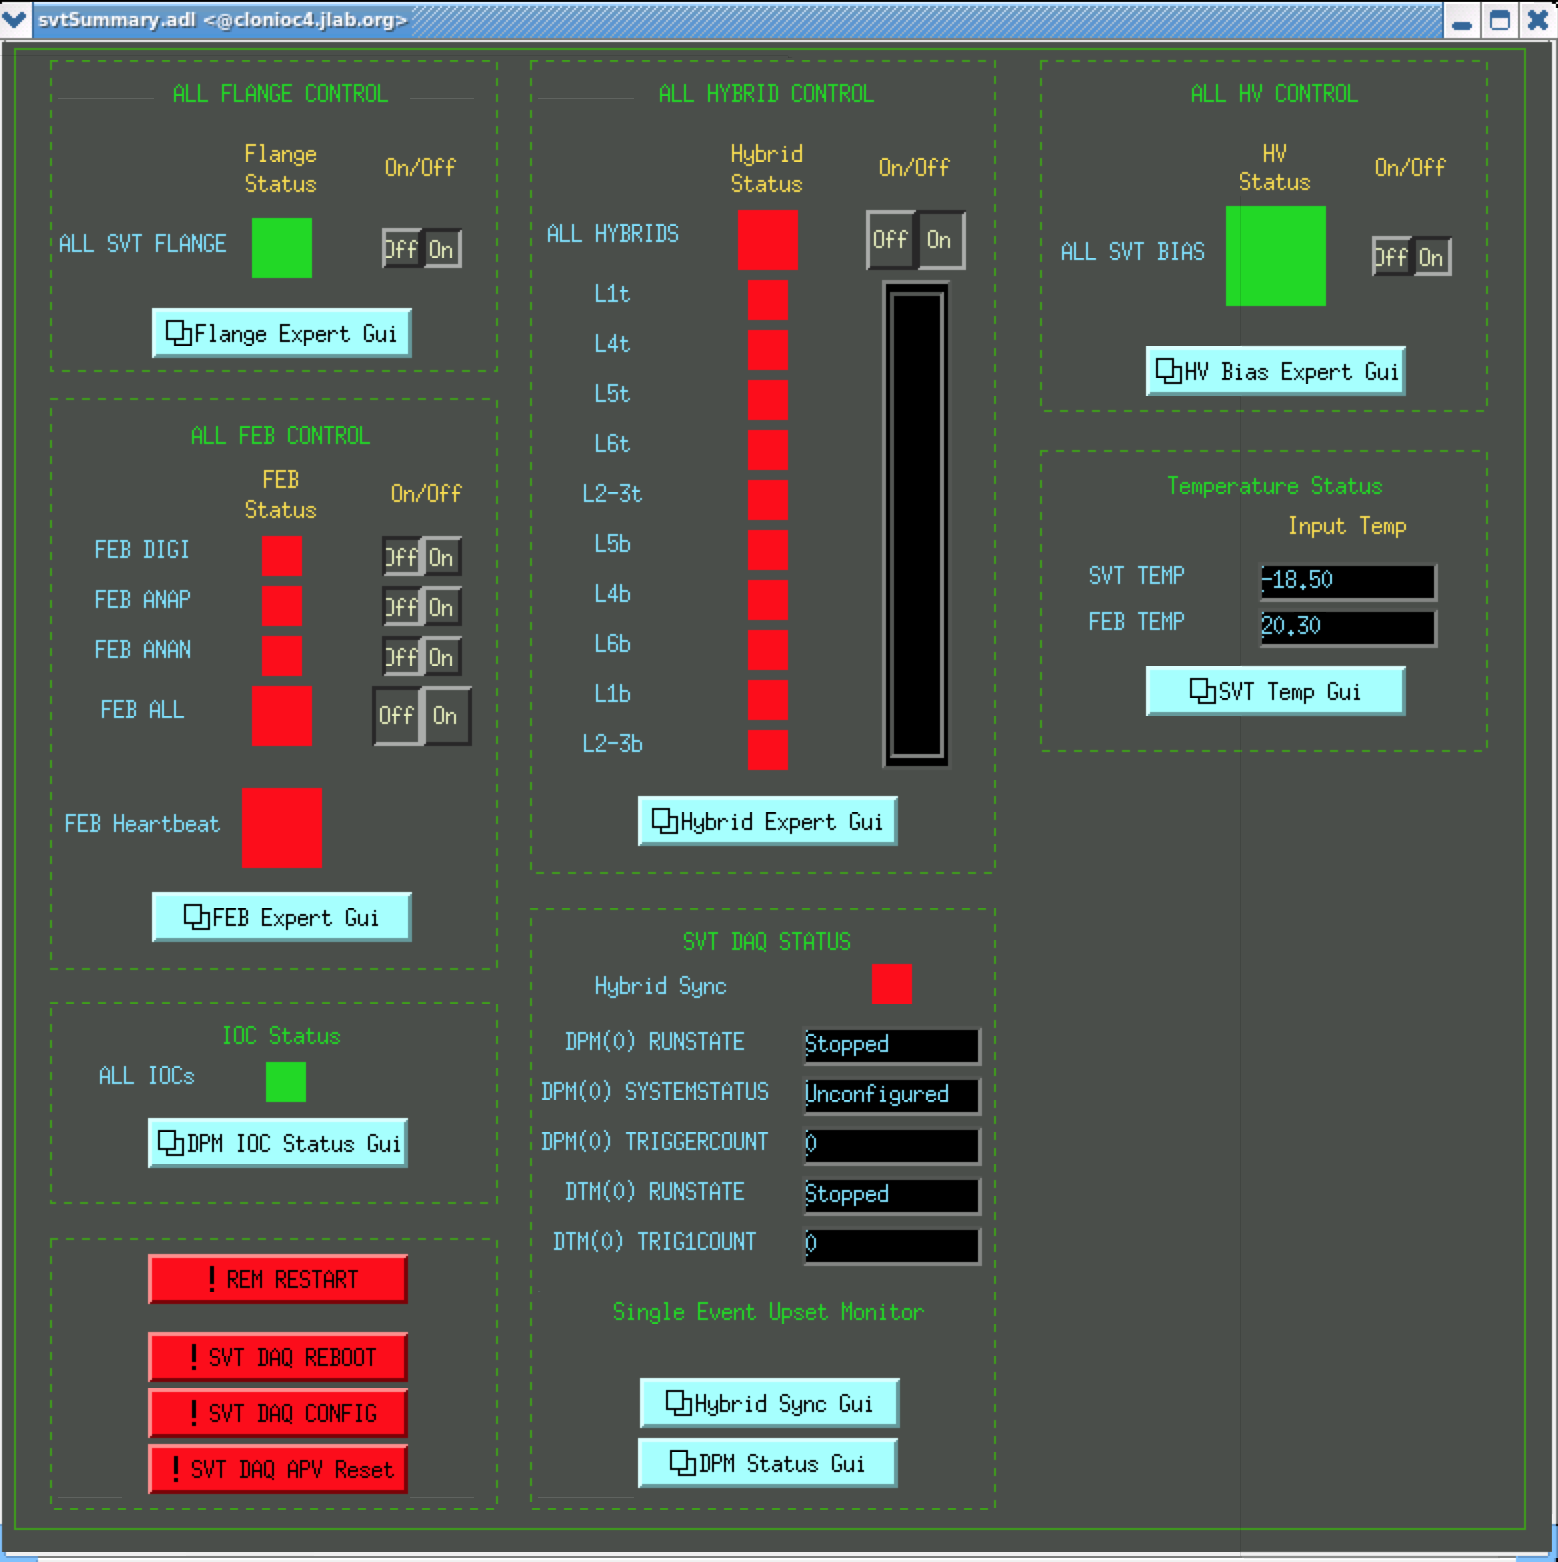
\includegraphics[width=\textwidth]{svt_summary_gui.png}
\caption{SVT summary GUI.}
\label{fig:svt_summary_gui}
\end{center}
\vspace*{-5mm}
\end{figure}
%=======================
\begin{enumerate}

\item
SVT position is appropriate for the run. 

\item 
High voltage bias is ON and at  180V (unless SVT expert  or run coordinator has told you something different). 
\newline NOTE: If the the HV is OFF and won't come on you might need to go and reset the interlock by going to the \texttt{Devices/SVT Soft Interlocks} GUI and Reseting the MPOD interlock. This happens after a beam trip. 
\newline {\bf \textcolor{red}{Important: Check that beam conditions for turning on bias voltage is OK before switching on!}}


\item 
FEB Status

\begin{enumerate}

\item
Under section \texttt{"ALL FEB CONTROL"} check that the status of \texttt{FEB ALL} is GREEN.

\item
Under section \texttt{"ALL FEB CONTROL"} check that the status of \texttt{FEB Hearbeat} is GREEN.

\end{enumerate}

\item 
IOC status

\begin{enumerate}

\item
Under section \texttt{"IOC Status"} check that the status of \texttt{ALL IOCs} is GREEN.

\end{enumerate}


\item Hybrid status

\begin{enumerate}

\item
Under section \texttt{"ALL HYBRID CONTROL"} check that the status of \texttt{ALL HYBRIDS} is GREEN.

\end{enumerate}

\end{enumerate}



\item
 \textcolor{red}{ {\bf If continuing with same the same run configuration from a stopped run continue to \ref{item:prestart}.}}

\item
In the \texttt{RunControl} GUI: click \texttt{connect}, the GUI should update with new windows. 

\item
Click on \texttt{Configure} in the transition section, choose configuration \texttt{'HPS35}. Click OK.
\item
\begin{enumerate}
\item
Check that \texttt{run number}, \texttt{data file path} and \texttt{run configuration} filename shown in the updated GUI make sense. 
\item
The \texttt{download} button should appear. 
\end{enumerate}


\item
\label{item:download}
Press \texttt{Download}.

\begin{enumerate}

\item
A popup window should appear to choose the trigger file, which should be defined in the run plan in the short term schedule on the HPS Run Wiki and/or the whiteboard in the counting house.

\item
Wait until the \texttt{Prestart} button appears and  \texttt{RunControl} GUI reports that Download was completed.\newline 
This might take up to 30s to complete.

\end{enumerate}

\item
Check SVT status

\begin{enumerate}

\item
In the \texttt{SVT summary GUI} under section \texttt{SVT DAQ STATUS} and check that both \texttt{DPM RUNSTATE}  \texttt{DPM RUNSTATE}  are saying \texttt{Download}.

\item
In the \texttt{SVT summary GUI} under section \texttt{ALL HYBRID CONTROL}, check that \texttt{ALL HYBRIDS} status is \texttt{GREEN}.

\end{enumerate}

\item
\label{item:prestart}
Press \texttt{Prestart} 

\begin{enumerate}

\item
Wait for the message ofl \texttt{Prestart succeeded}  in RunControl GUI\newline
This can take up to 30 seconds.

 \item
 The \texttt{Go} button should appear.

\item 
Check ECAL status
\begin{enumerate}
%Push the ``Manual Update'' button in the DIAG GUI a few times. The ``Cluster Latency'' plot should show a single spike. If it shows two spikes, issue the following command on clondaq5:\newline
%\texttt{> tcpClient hps11 'tiSyncReset()'}\newline
\item Check that FADC scaler rates are reasonable by comparison with a previous run with a similar trigger.  Sharp, odd patterns are a sign of misconfiguration.
\end{enumerate}


\item
Check SVT status

\begin{enumerate}

\item
In the \texttt{SVT summary GUI} under section \texttt{SVT DAQ STATUS} and check that both \texttt{DPM RUNSTATE}  \texttt{DPM RUNSTATE}  are saying \texttt{Prestart}.

\item
In the \texttt{SVT summary GUI} under section \texttt{SVT DAQ STATUS} and check that both \texttt{Hybrid Sync} status is \texttt{GREEN}.


\end{enumerate}

\end{enumerate}



\item
\label{item:go}
Press \texttt{Go} to start the run. 

\begin{enumerate}

\item
Wait for \texttt{transition Go succeeded}' message in the RunControl GUI.\newline
This can take about 10 seconds.

\item
The \texttt{End run} button should appear.

\item
Check that the run status is \texttt{running} and that triggers are issued at the expected rate.


\item
In the \texttt{SVT summary GUI} under section \texttt{SVT DAQ STATUS} and check that both \texttt{DPM RUNSTATE}  and \texttt{DPM RUNSTATE}  are saying \texttt{Go}.

\item
In the \texttt{SVT summary GUI} under section \texttt{SVT DAQ STATUS} and check that both \texttt{DPM TRIGGERCOUNT} and   \texttt{DTM TRIG1COUNT}  are incrementing.


\item
Reset the ECal and SVT monitoring plots (connect). 

\item
Check SVT occupancy and max sample plots.

\item
Fill out a row in the run spreadsheet. Check the whiteboard and run plan wiki for any other logging requirements.

\end{enumerate}
\end{enumerate}

\subsection{Stopping a run}

\begin{enumerate}

\item
\label{item:stop}
Press \texttt{End Run} in the \texttt{RunControl}  GUI to stop data taking.

\begin{enumerate}

\item
Wait for \texttt{End run succeeded} message in RunControl window. \newline
This can take about 15 seconds.

\item
The \texttt{Prestart} button should appear.

\item
In the \texttt{SVT summary GUI} under section \texttt{SVT DAQ STATUS} and check that both \texttt{DPM RUNSTATE}  and \texttt{DPM RUNSTATE}  are saying \texttt{Stopped}.


\end{enumerate}
\end{enumerate}


\subsection{Beam trips: actions and recovery for DAQ}

\begin{verbatim} THIS NEEDS TO BE UPDATED \end{verbatim}

Beam trips are frequent and in the most normal case the SVT high voltage bias will trip and will need to be restored before continuing.  If a beam trip happens:
\begin{enumerate}

\item When beam is back and we are ready (check BPM strip charts/scaler GUI to see that 2H02 position is back to normal) go to the SVT Bias GUI. Push the ``RESET'' button to reset the beam interlock, and push the ``180V'' button to ramp bias up to 180 V.

\item Reset the SVT monitoring plots (disconnect and connect). Check the occupancy and max sample plots.

\end{enumerate}


\newpage
\subsection{FIX DAQ}


\subsubsection{What to do if you get an Error During Download}

\begin{enumerate}
    \item In run control GUI: {\em Cancel} and then {\em Download}
    \item If still fails:
    \begin{enumerate}
    	\item Try to identify which of the ROCs (in the Runcotrol GUI message window or in the individual ROC windows) has a problem. 
        \item If only ONE of the TI, GTP or FADC indicates a problem, it may be possible to just restart it's process in Appendix~\ref{sec:codacommands}.  If more than one, just GOTO Section \ref{fixdaqbig}.
	\item If TI, GTP or FADC are OK but any of the 'dpm' or 'dtm' has problem, this might mean only the SVT DAQ is in a bad state: GOTO Sec.~\ref{fixsvtdaq}
    \end{enumerate}
    \item GOTO Step \#9 in Section \ref{sec:startstop}.
\end{enumerate}

\subsubsection{What to do if you get an Error During Prestart}

\begin{enumerate}
	\item Try to identify which of the ROCs (in the Runcotrol GUI message window or in the individual ROC windows) has a problem.
	\item Check specifically in the ROC windows for the 'dtm0' and 'dtm1'. If they are the only ROCs that got killed and they show an error saying that they cannot get "Run state" then
	\begin{enumerate}
	    	\item In the ROC xterm window: restart the roc process, typically hit up arrow on keyboard and press enter.
		 \item In run control GUI: {\em Cancel} and then {\em Download} and continue from there.
		 \item If it happens more than 3 times in a row, report the status of the roc window in dpm7 and contact SVT expert
	 \end{enumerate}
	 \item GOTO Step \#9 in Section \ref{sec:startstop}.
\end{enumerate}


\subsubsection{Full DAQ Reboot}
\label{fixdaqbig}

\begin{enumerate}
\item Reboot the master TI and ECal DAQ by executing this command in a terminal:
\newline
\centerline{\texttt{hpsRocRebootAll.sh}}
This will reboot hps11, hps12, hps1, and hps2, and then wait for a ping response from hps2, meanwhile giving some progress messages.  When finished it will display ``DAQ FIXED'' in the terminal.

\item Reboot the SVT DAQ: GOTO Sec.~\ref{fixsvtdaq}

\end{enumerate}

%    \item These two commands can be done in parallel (simultaneously) in two different terminals and will gradually kill all the terminals in Figure~\ref{fig:coda}.  Do not wait for them to finish before proceeding to the next step.
%      \subitem \texttt{hps\_exit}
%      \subitem \texttt{roc\_xterms\_exit}
%    \item \texttt{roc\_reboot hps11}
%    \item Wait 30 seconds, then reboot the rest of the ROCs (these can all be done in parallel):
%      \subitem \texttt{roc\_reboot hps1}
%      \subitem \texttt{roc\_reboot hps2}
%      \subitem \texttt{roc\_reboot hps12}
%    \item Confirm Successfull Login to all ROCs (and logout afterwards): 
%        \subitem\texttt{ssh hps11, hps12, hps1, hps2, hps1gtp, hps2gtp}
%        \subitem This will not work instataneously; keep trying until all the ROCs are fully alive.  Should not be more than a couple minutes.  Pings will work before sshes.  If any fail to ssh successfully without error after 5 minutes, reboot the culprit ROC.  {\em If you need to rereboot hps11 here, GOTO STEP \#2}.
%    \item After all 6 sshs are succesful and Step \#1 has completed, do the following.  These can be done in parallel in two different terminals:
%    \subitem \texttt{hps\_start}
%    \subitem \texttt{roc\_xterms\_start}
%    \item After rebooting ROCs, you may have to reboot the trigger scalers GUI (REBOOT button at the bottom right).
%\item GOTO Step \#5 in Section \ref{sec:startstop}
%
%
%\end{enumerate}


\subsubsection{Debugging deadtime}


\begin{verbatim} THIS NEEDS TO BE UPDATED \end{verbatim}



If you start a run and see an event rate of under 1 Hz and a livetime of 0\%:
\begin{enumerate}
\item On any clon,\newline
\texttt{> tcpClient hps11 tiStatus}\newline
\item Look for ``BUSY input source'':

\begin{tabular}{ l|l }
  HFBR \# & ROC and system \\
  1 & hps1 (ECal) \\
  2 & hps2 (ECal) \\
  3 & hps12 (ECal) \\
  4 & SVT DAQ \\
  5 & SVT DAQ \\
\end{tabular}
\item Do a full DAQ teardown, rebooting the problem ROC (if SVT DAQ, do a FIX SVT DAQ including \texttt{rem\_restart.sh})
\end{enumerate}









\subsubsection{FIX SVT DAQ}
\label{fixsvtdaq}

\textcolor{red}{
Before following the below procedure, please record in a log entry the answer to these questions to help us debug and improve the DAQ:
\begin{itemize}
\item What is the status of CODA: Did any of the ECAL ROCs crash? Did the EB, ET or ER crash? 
\item When did it fail: In state transition  'Download',  'Prestart'  or 'Go' or during a run?
\item What is the status of the ROCs (There are 14 DPMs and 2 DTMs): did they crash or report any error message?
\item Open the \texttt{/SVT/DAQ IOC Status} GUI and write down the status: which ones are red/green?
\end{itemize}
}



The procedure below is a full reboot of the SVT DAQ and may take up to 2 minutes to finish. 

\begin{enumerate}

\item
In the \texttt{SVT summary GUI}, bottom left section, click the \texttt{SVT DAQ REBOOT} button.

\item
A new x terminal should popup. If it asks for a password it's the same as for user \texttt{clasrun} or \texttt{hpsrun}.

\item
The terminal will print out status of the reboot and will not close after finishing. You have to manually close it. \newline
This may take up to 2 minutes.\newline
\textcolor{red}{While rebooting the SVT crate the ssh process can hang while halting DAQ nodes. If this happens it will get stuck one one or a few nodes in the beginning of the process. If it happens, wait 15 seconds before hitting {\em Cntrl-c} and the process should continue to the next. }

\item 
After a successful finish, go to the the \texttt{SVT summary GUI}, and look for any errors following the check list starting from item~\ref{item:svt-checklist} in ~Sec~\ref{sec:startstop}.

\item
In case of failure, copy the output of the x terminal into a logbook post and call the expert.


%\begin{enumerate}
%    \item If one or many of the DPMs failed to or prestart
%	\begin{enumerate}
%    		\item Reboot the software by login into  \texttt{clondaq5} as 'clasrun'. \newline
%		\texttt{> cd $\$$CLAS/slac\_svt/svtdaq/daq/rceScripts} \newline
%		\texttt{> ./rem\_restart.sh} \newline
%		You will see the script connecting to each host. Wait until finished, can be up to 20s. \newline
%		Wait until you can ping host 'dtm0' \newline
%		Open the \texttt{/SVT/DAQ IOC Status} GUI and verify that the control DPMs are green; it may take up to 30s (the FEBs need to be powered).
%		\item Go back to the run control GUI and repeat the 'Download' step (may need to 'Cancel' and 'Reset' first)
%		\item If one or many DPMs are still having issues then reboot the "COB"  by login into  \texttt{clondaq5} as 'clasrun'. \newline
%		\texttt{> cd $\$$CLAS/slac\_svt/svtdaq/daq/rceScripts} \newline
%		\texttt{> ./reboot\_cob} \newline
%		Wait at least 10s. \newline
%		Make sure you can ping host 'dtm0' \newline
%		Repeat:\newline
%		\texttt{> ./reboot\_cob} \newline
%		Wait at least 10s. \newline
%		Make sure you can ping host 'dtm0' \newline
%		Open the \texttt{/SVT/DAQ IOC Status} GUI and verify that the control DPMs are green; it may take up to 30s (the FEBs need to be powered). The data DPMs might be red until you go past to 'Download'.
%
%		\item After rebooting DPMs or COBs, hybrids will be turned off. Don't forget to switch them back on after the ``Download'' step.
%		
% 	\end{enumerate}
%\end{enumerate}


\end{enumerate}


    
   
\section{Detailed SVT checklist}

\begin{enumerate}
\item 
SVT Flange boards (\texttt{SVT/Flange} GUI) and SVT Front end boards (\texttt{/SVT/FEB Main} GUI) are powered  with no alarms. 
\newline
{\bf IF ON:} check that currents are updating: if not, try to reboot the "iochvCaen" IOC.
\newline
{\bf IF OFF:} 
\begin{enumerate}
\item 
Restart the FEBs turning on in the order: 1) 'DIGI', 2) 'ANAP' and then 3) 'ANAN'; buttons are at the top of the \texttt{/SVT/FEB Main} GUI.
\item
Power all the flange channels from   \texttt{SVT/Flange}  GUI. 
\item 
Go to the \texttt{/SVT/Link Status} GUI and check that no FEB link errors are stably incrementing. If they do, try to cycle the flange board power (wait 10-20s between cycles). You may need up to 4 cycles.
\end{enumerate}
\item 
Bias high voltage is ON and at 180V (unless SVT expert has told you something different). 
\newline If the the HV is OFF and won't come on you might need to go and reset the interlock by going to the \texttt{Devices/SVT Soft Interlocks} GUI and Reseting the MPOD interlock. This happens after a beam trip. 
\newline {\bf \textcolor{red}{Important: Check that beam conditions for turning on bias voltage is OK before swiching on (see above)!}}

\item
SVT DAQ is in a state ready to run:
\begin{enumerate}
\item
Check that all the Control and Data DPMs and DTMs in \texttt{SVT/DAQ IOC Status} GUI are OK. 
\newline NOTE1: If there was a reboot of the SVT DAQ software or COB (see below) the data DPMs might not show green until after the 'Download' transition. 
\newline NOTE2:The control DPM should be OK as soon as a single FEB (and flanges are powered). It might take up to 30s for it to become green.

\item
Check that error counts in the \texttt{SVT/svtDpmLinkStatus} GUI are zero and not updating.

\item
In \texttt{/SVT/DPM Status} GUI": check that all data DPMs are in the appropriate CODA Run state e.g. if you are in 'Download' all should be in that state, etc. 
\newline NOTE: This may be not updated if there was a DAQ restart, e.g. the DPMs might be in 'End' as they doesn't know that CODA was restarted until 'Download' is initiated.
\end{enumerate}
\end{enumerate}




%=======================
\begin{figure}[htbp]
\begin{center}
    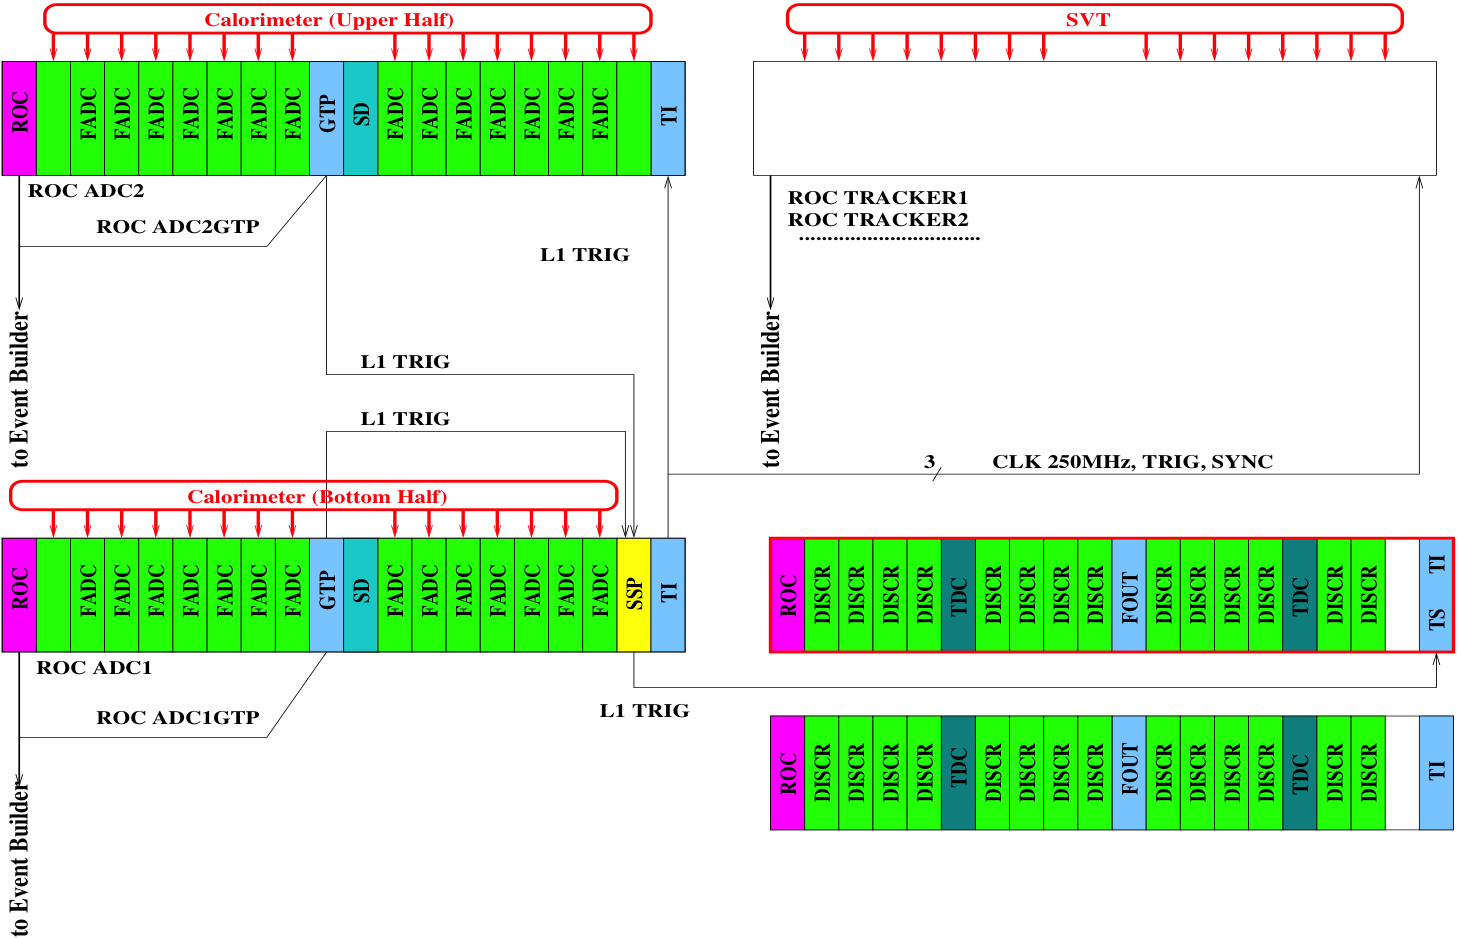
\includegraphics[width=\textwidth]{daq.png}
\caption{Schematic overview of the DAQ and trigger system.}
\label{fig:daq}
\end{center}
%\vspace*{-5mm}
\end{figure}
%=======================

\newpage

\appendix
\section{Chaning Prescale Factors on the Fly}
This script will change the prescale factors immediately (during a run) and update the EPICS prescales
such that the trigger GUI always uses the active prescales:\newline
\centerline{\texttt{hpsTiPrescale.sh TRIGGER PRESCALE}}


\appendix
\section{Rebooting an Individual ROC}\label{sec:rebootaroc}
Execute this command (where \texttt{ROC} is one of \texttt{hps11, hps12, hps1, hps2}):\newline
\centerline{\texttt{roc\_reboot ROC}}

\vspace{5mm}\noindent
*Note that \texttt{hps1gtp} lives in \texttt{hps1}, so rebooting \texttt{hps1gtp} is done via \texttt{roc\_reboot hps1} (and similarly for \texttt{hps2gtp}).

\vspace{5mm}\noindent
{\em IF YOU REBOOT \texttt{hps11}, YOU MUST WAIT 30 SECONDS AND SUBSEQUENTLY REBOOT ALL OTHER ROCS \texttt{hps1, hps2, hps12} BEFORE PROCEEDING}.

    After rebooting ROCs, you may have to reboot the trigger scalers GUI (REBOOT button at the bottom right).
\section{Restarting Individual CODA Processes}\label{sec:codacommands}
If a CODA command dies (returns to prompt in the corresponding terminal) or a ROC must be rebooted, the CODA command for that ROC must be restarted.  The command can be manually executed again in the same terminal it was initally running in without a full DAQ restart.

If the ROC was not rebooted and only the CODA command died, the command should be the most recent in the shell history.  In this case you you should be able to press {\em up} in the terminal and re-execute the command.

Alternatively, this command will start the appropriate CODA process for the host it is run on:

\centerline{\texttt{hpsRocStart.sh}}

%Otherwise, here is a list of the CODA commands to be run on each ROC.  These should be executed in a terminal that is logged into the appropriate ROC (\texttt{hps1, hps2, hps11, hps12, hps1gtp,or hps2gtp}) as user \texttt{clasrun}.
%\begin{itemize}
%    \item \texttt {coda\_roc\_gef -s clashps -o $''$hps11 TS$''$}
%    \item \texttt {coda\_roc\_gef -s clashps -o $''$hps12 ROC$''$}
%    \item \texttt {coda\_roc\_gef -s clashps -o $''$hps1 ROC$''$}
%    \item \texttt {coda\_roc\_gef -s clashps -o $''$hps2 ROC$''$}
%    \item \texttt {coda\_roc -s clashps -o $''$hps1gtp ROC$''$}
%    \item \texttt {coda\_roc -s clashps -o $''$hps2gtp ROC$''$}
%\end{itemize}

\end{document}
